%
% Positronium-hydrogen Kohn variational method scattering paper
%

%\documentclass[preprint,showpacs,showkeys,preprintnumbers,amsmath,amssymb,longbibliography,pra,aps,superscriptaddress]{revtex4-1}
\documentclass[preprint,showpacs,showkeys,preprintnumbers,amsmath,amssymb,longbibliography,pra,aps]{revtex4-1}
%\documentclass[reprint,showpacs,preprintnumbers,amsmath,amssymb,pra,aps,longbibliography]{revtex4-1}

% Denton's shortcuts
\newcommand{\ee} {\,\text{e}}
\newcommand{\ii}{{\rm{i}}}

% Packages

\usepackage{graphicx}  % Include figure files
%\usepackage[draft]{graphicx}  % Do not include figure files
\usepackage{dcolumn} % Align table columns on decimal point
\usepackage{bm} % bold math
\usepackage{float}  % @TODO: Take this out before submission!
\usepackage{todonotes}
\usepackage[hidelinks]{hyperref}  % For clickable references
\usepackage{amssymb}
\usepackage{xcolor}
\usepackage{wasysym}  % Simply for \CIRCLE and \Circle (could use \circ for the latter)
\usepackage[normalem]{ulem}  % Remove this - strikethrough text

\usepackage{silence}
\WarningFilter{revtex4-1}{Repair the float}  % Completely innocuous warning - http://tex.stackexchange.com/questions/180762/revtex4-1-warning-repair-the-float-package

% Subfolders containing our images
\graphicspath{{IPython/}{Images/}}

% Remove before submitting
\newcommand{\todoi}{\todo[inline]}

% To center table head
\newcommand*{\thead}[1]{\multicolumn{1}{c}{#1}}

\setlength{\abovecaptionskip}{0pt}  % Reduce space between figure and caption (default of 10pt)
\setlength{\paperheight}{11in}  % To get rid of the annoying hyperref warning


\begin{document}

%\preprint{APS/123-QED}

\title{An Investigation of Low-Energy Positronium-Hydrogen Scattering}

\author{Denton Woods}
\email{denton.woods@unt.edu}
\homepage{http://www.dentonwoods.com}

\author{S. J. Ward}
\affiliation{Department of Physics, University of North Texas, Denton, Texas 
76203, USA}

\author{P. Van Reeth}
\affiliation{Department of Physics and Astronomy, University College London, 
Gower Street, London WC1E 6BT, UK}

\date{\today}

\begin{abstract}
We investigate the four-body Coulomb process of low-energy elastic
positronium-hydrogen (Ps-H) scattering below the Ps(n=2) excitation threshold
with a Hylleraas-type basis set. Using the complex Kohn variational method, we 
compute phase shifts through the $^{1,3}F$-wave. The $^{1,3}S$- and
$^{1,3}P$-wave phase shifts can be viewed as benchmark results. The complex
Kohn variational results compare well to a number of other calculations for 
this system. Using the Hylleraas-type basis set, we also compute the binding 
energy of $^1S$ positronium hydride. In addition, we present elastic 
differential, elastic integrated, momentum transfer, and ortho-para 
conversion cross sections, and for the singlet, resonances through the
$F$-wave. Finally, we give a detailed analysis of the scattering lengths
and effective ranges using multiple effective range theories.
\end{abstract}

   
\pacs{31.15.xt Variational techniques; 34.50.-s Scattering of atoms and
molecules; 36.10.Dr Positronium; 34.80.Bm Elastic scattering}
\keywords{positronium; PsH; positronium hydride; Kohn variational}
\maketitle

\section{\label{sec:Intro}\protect Introduction}


%\preprint{APS/123-QED}

Positronium (Ps) scattering from atoms and molecules is an area of current 
experimental and theoretical interest. The development of energy-tunable
ortho-Ps beams
\cite{Brown1985,Laricchia1987,Zafar1996,Garner1996,Laricchia2008} 
has enabled measurements to be made of Ps scattering from the inert gases He,
Ne, Ar, Kr, and Xe
\cite{Garner1996,Garner2000,Armitage2002,Laricchia2004,Armitage2006,Laricchia2008,Engbrecht2008,Brawley2010a}
and the molecules H$_2$, N$_2$, O$_2$, CO$_2$, H$_2$O, and SF$_6$
\cite{Garner1996,Garner1998,Garner2000,Laricchia2004,Armitage2006,Beale2006,Brawley2010a}.
Cross sections for Ps scattering from H have not been measured due to the
difficulty of an atomic hydrogen beam, although the binding energy of positronium
hydride (PsH) has been measured in the reaction of a positron with methane,
e$^+$ + CH$_4$ $\to$ CH$_3^+$ + PsH \cite{Schrader1992}. The low-energy region
is of particular interest, because in this energy range, positron and electron 
correlations are dominant. We present
\cite{Conferences1,Conferences2,Conferences3,WoodsDiss2015} 
our work of the application of the complex Kohn variational 
method to elastic Ps(1s)-H(1s) scattering in the energies up to the 
excitation threshold of Ps(n=2) at 5.101 eV.

Ps-H scattering is a fundamental four-body Coulomb process. The Kohn (and 
inverse Kohn) variational method has previously been applied to Ps-H 
collisions by Van Reeth and Humberston \cite{VanReeth2003,VanReeth2004}, who 
computed $^{1,3}S$ and $^{1,3}P$ elastic phase shifts. We 
have extended their $^{1,3}S$ and $^{1,3}P$ Kohn variational calculations in 
multiple ways. First, and foremost, in addition to implementing
the Kohn and inverse Kohn variational methods, we have implemented the 
generalized Kohn, the complex Kohn for the $S$ and $T$ matrices, and the
generalized complex Kohn for the $S$ and $T$
matrices. The complex Kohn variational methods are known to suffer
from far fewer anomalous singularities than the Kohn, inverse Kohn and 
generalized Kohn variational methods
\cite{Lucchese1989, Cooper2009, Cooper2010}. The second extension that we
consider is to use the procedure by Todd 
\cite{Todd2007} to systematically remove short-range terms that cause linear 
dependence. This enables us to compute the phase shifts (and the binding 
energy of PsH) with more short-range Hylleraas terms than the earlier 
Kohn calculations. We add the asymptotic expansion of Drake and Yan
\cite{Drake1995, Yan1997} to improve the accuracy of the short-range
integrations. We have also significantly increased the number of integration
points for matrix
elements that involve the long-range terms, along with implementing a method to
accelerate the convergence of these integrals. We also extend the 
calculations to the next two partial waves through to the $F$-wave, which
enables us to calculate the differential elastic, integrated elastic, momentum
transfer, and ortho-para conversion cross sections.

We present results in this paper obtained using the $S$ matrix complex Kohn 
variational principle for Ps-H scattering. We confirm the previously observed 
resonances for the first four partial waves and compare the positions and 
widths to that of the earlier Kohn \cite{VanReeth2003,VanReeth2004}, close 
coupling (CC) \cite{Walters2004} and complex rotation calculations
\cite{Yan1999,Yan1998a,Ho1998,Ho2000}. In addition, we compute the scattering
lengths and effective ranges using multiple effective range theories.

We also use the short-range part of the full scattering wavefunction to 
compute the binding energy of PsH. Comparing the binding energy with the most 
elaborate variational results gives an indication of the reliability of 
describing the Ps-H system at short distances. The binding energy of PsH,
$E_b$, has been calculated using various methods. Ho \cite{Ho1986} performed a 
variational calculation with a Hylleraas basis set, and Yan and Ho
\cite{Yan1999} later did a more extensive calculation. Mitroy \cite{Mitroy2006}
used the stochastic variational method (SVM) with 1800 explicitly correlated 
Gaussians (ECGs), and Bubin and Adamowicz \cite{Bubin2006} found the most 
accurate value using 5000 ECGs in a variational calculation.

There have been a number of other calculations for Ps-H scattering. A much 
earlier Kohn variational calculation was performed by Page \cite{Page1976} 
for the Ps-H scattering lengths. Drachman and Houston used a stabilization 
method with an effective range theory (ERT) expansion
\cite{Drachman1975,Drachman1976}. At low energies, diffusion Monte Carlo (DMC)
\cite{Chiesa2002}, the SVM \cite{Ivanov2001,Ivanov2002}, CC
\cite{Sinha1997,Campbell1998,Adhikari1999,Sinha2000,Blackwood2002,Blackwood2002b,Walters2004},
static exchange \cite{Hara1975,Ray1997}, and Kohn variational
\cite{Page1976,VanReeth2003,VanReeth2004} methods have been applied. The SVM
with stabilization 
techniques was used to compute low-energy phase shifts and 
scattering lengths for Ps-H collisions \cite{Ivanov2001,Ivanov2002}.

Blackwood et al.~\cite{Blackwood2002} performed an elaborate CC calculation 
for Ps scattering from H, which took into account excitation and ionization 
of both the projectile and target. They considered two different coupling 
schemes. The first one, which they refer to as 9Ps9H, included 9 eigen- and 
pseudo-states of Ps and also of H. The second scheme, which they refer to as 
14Ps14H, is for the singlet only and includes 14 eigen- and pseudo-states of 
Ps and also of H. Good agreement is obtained between the CC
\cite{Blackwood2002} and the SVM \cite{Ivanov2002} for the $S$-wave scattering
lengths and phase shifts. In another paper, Blackwood et
al.~\cite{Blackwood2002b} considered the importance of including the H$^-$
channel in a 22Ps1H coupling scheme, comparing to the previous 22Ps1H
calculations of Campbell et al. \cite{Campbell1998}. Walters et
al.~\cite{Walters2004} extended the earlier CC calculations
\cite{Blackwood2002} to include the e$^+$-H$^-$ channel
\cite{Blackwood2002b} and compared their results for the $S$-wave with the
accurate Kohn variational results \cite{VanReeth2003}. They speculated that the
inclusion of the virtual Ps$^-$ formation channel may be needed to obtain 
agreement with the Kohn variational results for Ps(1s)-H(1s) scattering 
\cite{Blackwood2002}. A recent calculation of Ps-H scattering uses the
confined variational method (CVM) \cite{Zhang2012}. This provides accurate
results but has the drawback of being very computationally expensive. In
Ref.~\cite{Zhang2012}, Zhang and Yan calculate phase shifts for 2 momenta for
both $^1S$ and $^3S$.

Unlike the SVM and DMC methods, the Kohn variational method gives rigorous 
bounds on the scattering lengths and, except for Schwartz singularities, 
gives empirical bounds on the elastic phase shifts. This means that the wave 
function can be systematically improved to the converged results. The Kohn 
variational method is known to yield accurate results and has provided 
benchmark results \cite{VanReeth2003,VanReeth2004} to which results from 
other calculations can be compared. %\sout{Unlike the SVM, the Kohn variational
%method can treat inelastic as well as elastic scattering and thus can be 
%extended to higher energies.}

Phase shifts are expressed in radians. Atomic units are used throughout 
unless otherwise stated. For conversions to electron-volts (eV), we use the 
conversion factor 1 a.u. = {27.21138505(60) eV}
\cite{Mohr2012,*NISTConversions}.

%\emph{Add \cite{Shipman2014}, \cite{Barker2012}, \cite{Laricchia2009}?}
%\emph{Add \cite{Mitroy2002a}?}


\vskip 0.5truecm
\noindent
\section{Theory}

\subsection{The Positronium-Hydrogen System}
\begin{figure}[H]
	\centering
	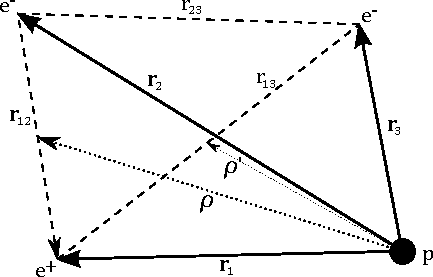
\includegraphics[height=2in]{PsHCoordinates}
	\caption{Positronium-hydrogen coordinate system}
	\label{fig:PsHCoords}
\end{figure}

We are investigating low-energy elastic scattering of ground-state Ps
with ground-state 
hydrogen, Ps(1s)+H(1s), for incident energies up to the excitation threshold 
of Ps(n=2)+H(1s), which is at an energy of $\tfrac{3}{16}$ a.u. ($5.102$ eV). 
Previous work on Ps-H scattering used the Kohn and inverse Kohn variational
methods \cite{VanReeth2003, VanReeth2004}. The complex Kohn variational
methods are more stable and
suffer less from Schwartz singularities than the Kohn, inverse Kohn and 
generalized Kohn methods \cite{Lucchese1989,Cooper2009,Cooper2010}. 
Van Reeth and Humberston \cite{VanReeth1999} used the complex Kohn 
variational method for e$^+$-He scattering. The results we present in Sec.
\ref{sec:Results} use the $S$ matrix complex Kohn variational method,
but we present in
this section a general wavefunction that can be used in any of the variants
of the Kohn variational method, as we describe in Sec. \ref{sec:Kohn}.
We use the variants of the Kohn variational method to obtain estimates
of errors associated with the phase shifts, resonance parameters, and
scattering lengths. Also, importantly, we feel that it is elegant to
have a single formulation for the Kohn variational method and its variants.

For $S$-wave Ps(1s)-H(1s) elastic scattering, the flexible scattering
wavefunction is given by
\begin{equation}
\Psi_0^{\pm,t} = \widetilde{S}_0 + L_0^{\pm,t} \, \widetilde{C}_0
  + \sum_{i=1}^{N(\omega)} c_{i0} \bar{\phi}_{i\ell 1},
\label{eq:TrialWave}
\end{equation}
where the superscript $t$ indicates that this is a trial wavefunction. The plus
sign indicates the spatially symmetric singlet case, and the minus sign
indicates the spatially antisymmetric triplet. The total orbital angular
momentum of the system is equal to the orbital angular momentum of the incoming
ground-state Ps, $\ell$. For partial waves $\ell > 0$, we consider a trial
wavefunction of the form
\begin{equation}
\Psi_\ell^{\pm,t} = \widetilde{S}_\ell + L^{\pm,t}_\ell \, \widetilde{C}_\ell
 + \sum_{i=1}^{N(\omega)} c_{i\ell} \bar{\phi}_{i\ell 1}
 + \!\!\!\sum_{i=N(\omega)+1}^{2N(\omega)} \!\! d_{i\ell} \bar{\phi}_{i\ell 2}.
\label{eq:TrialWaveHigher}
\end{equation}
The scattering wavefunctions contain both the long-range terms $\bar{S}$ and
$\bar{C}$ and the short-range correlation terms $\bar{\phi}_{i\ell k}$ for
small interparticle distances. The 
long-range terms of Eqs. (\ref{eq:TrialWave}) and (\ref{eq:TrialWaveHigher})
are given by
\begin{equation}
\label{eq:SCPhiDef}
\begin{bmatrix}
\widetilde{S}_\ell \\ \widetilde{C}_\ell
\end{bmatrix} = \textbf{u}  \begin{bmatrix}
\bar{S}_\ell \\ \bar{C}_\ell
\end{bmatrix} = \begin{bmatrix}
u_{00} & u_{01} \\  u_{10} & u_{11}
\end{bmatrix}
\begin{bmatrix}
\bar{S}_\ell \\ \bar{C}_\ell
\end{bmatrix}, 
\end{equation}
with
\begin{subequations}
\label{eq:SCBarPhiDef}
\begin{align}
\bar{S}_\ell &= \frac{1\pm P_{23}}{\sqrt{2}}Y_{\ell 0}(\theta_\rho,
  \varphi_\rho)\Phi_{{\rm{Ps}}(1S)}\!\left(r_{12}\right) \Phi_{{\rm{H}}(1S)}\!\left(r_3\right)
  \sqrt{2\kappa} \,j_\ell\left(\kappa\rho\right) \text{ and} \label{eq:SBar} \\
\bar{C}_\ell &= -\frac{1\pm P_{23}}{\sqrt{2}}Y_{\ell 0}(\theta_\rho,
  \varphi_\rho)\Phi_{{\rm{Ps}}(1S)}\!\left(r_{12}\right) \Phi_{{\rm{H}}(1S)}\!\left(r_3\right)
  \sqrt{2\kappa} \,n_\ell\left(\kappa\rho\right) f_\ell(\rho). \label{eq:CBar}
\end{align}
\end{subequations}
Fig.~\ref{fig:PsHCoords} gives the
coordinate system for Ps-H. The vector
$\bm{\rho} = \frac{1}{2}\left(\bm{r_1} + \bm{r_2}\right)$ is the position
vector of the center of mass of the Ps atom with respect to the proton.
The $j_\ell\left(\kappa\rho\right)$ and $n_\ell\left(\kappa\rho\right)$ are
the spherical Bessel and Neumann functions, respectively.
$Y_{\ell 0}(\theta_\rho, \varphi_\rho)$ represents the spherical harmonics.
$P_{23}$ is the exchange operator for the two indistinguishable electrons.
$\Phi_{{\rm{Ps}}(1S)}\!\left(r_{12}\right)$ and
$\Phi_{{\rm{H}}(1S)}\!\left(r_3\right)$ are the ground-state wavefunctions
of Ps and H, respectively. The shielding factor, $f_\ell(\rho)$,
ensures that the singularity of the spherical Neumann function is removed
at the origin. We choose it to have the form
\begin{equation}
f_\ell(\rho) = \left[1 - \ee^{-\mu \rho} \left(1+\frac{\mu}{2}\rho\right)
\right]^{m_\ell}.
\label{eq:PartialWaveShielding}
\end{equation}
Table \ref{tab:Nonlinear} shows the values of the nonlinear
parameter $\mu$ and the integer $m_\ell$ we use for each partial wave.

We consider the Kohn variational method and a number of variants,
and $\textbf{u}$ and $L^{\pm}_\ell$ take
different forms depending on each. The $\textbf{u}$ matrices and
$L^{\pm,t}_\ell$ are given below:
\begin{subequations}
\label{eq:KohnU}
\begin{align}
&\text{generalized Kohn, } L^{\pm,t}_\ell = \tan(\delta^{\pm,t}_\ell-\tau),
 \textbf{u} = \left[ \begin{smallmatrix}
\cos \tau & \ \sin \tau \\  -\sin \tau & \  \cos \tau
\end{smallmatrix} \right], \label{eq:GenKohn}\\
&\text{generalized \emph{T} matrix Kohn, } L^{\pm,t}_\ell = T_\ell^{\pm},
 \textbf{u} = \left[ \begin{smallmatrix}
\cos\tau & \ \sin\tau \\ -\sin\tau + \ii \cos\tau & \ \cos\tau + \ii \sin\tau
\end{smallmatrix} \right], \text{and}\label{eq:GenTKohn} \\
&\text{generalized \emph{S} matrix Kohn, } L^{\pm,t}_\ell = S_\ell^{\pm},
 \textbf{u} = \left[ \begin{smallmatrix}
-\ii \cos\tau - \sin\tau & \ -\ii\sin\tau + \cos\tau \\ 
 \ii\cos\tau - \sin\tau & \ \ii\sin\tau + \cos\tau
\end{smallmatrix} \right]. \label{eq:GenSKohn}
\end{align}
\end{subequations}
For the case of $\tau = 0$, these give the Kohn, the \emph{T} matrix and
\emph{S} matrix complex Kohn variational methods, respectively.
$\tau = \frac{\pi}{2}$ in Eq. (\ref{eq:GenKohn})
gives the inverse Kohn. 
The \textbf{u} matrix for the generalized Kohn is identical to that given by
Cooper et al.\ \cite{Cooper2010}, and the \textbf{u} matrices for the
generalized complex Kohn methods are similar to Cooper et al. \cite{Cooper2010}.
The \textbf{u} matrices in Eq.~(\ref{eq:KohnU}) are similar to the
$\textbf{u}$ matrices given by Lucchese \cite{Lucchese1989} but are more 
generalized versions, and the \emph{T} matrix and \emph{S} matrix choices are 
slightly different. We use the definition of the \emph{T} and \emph{S} matrices
given by Bransden \cite{Bransden2003}.
Also, the \textbf{u} matrix for the inverse Kohn,
$\cot\delta_\ell^\pm$ differs from Lucchese \cite{Lucchese1989}.

The short-range terms are highly correlated Hylleraas-type functions, including
all interparticle distances, given by
\begin{equation}
\label{eq:PhiDef}
\bar{\phi}_{i\ell k} = \left(1 \pm P_{23}\right) Y_{\ell 0}(\theta_k,\phi_k)
e^{-(\alpha r_1 + \beta r_2 + \gamma r_3)}
r_k^{\ell} r_1^{k_i} r_2^{l_i} r_{12}^{m_i} r_3^{n_i} r_{13}^{p_i} r_{23}^{q_i}.
\end{equation}
The variable $\omega$ is a non-negative integer that determines the maximum
number of terms in the basis set. For a chosen value of $\omega$, the integer
powers of $r_i$ and $r_{ij}$ are constructed in such a way that 
%\todoi{Think about doing $r_i$ and $r_{ij}$ with different subscripts}
\begin{equation}
k_i + l_i + m_i + n_i + p_i + q_i \leq \omega,
\end{equation}
with all $k_i, l_i, m_i, n_i, q_i$ and $p_i \geq 0$.
The first set of short-range terms in Eq. (\ref{eq:TrialWaveHigher}), which we
refer to as the first symmetry, has $k=1$ for $i=1$ to $N(\omega)$. The second
symmetry set of terms exists for $\ell > 0$, with $k=2$ and $i = N(\omega)+1$
to $2N(\omega)$. These short-range terms represent the angular momentum as being placed on 
either the positron ($r_1$) or on the electron on the Ps atom ($r_2$, and $r_3$
with exchange). Following up on Ref. \cite{VanReeth2004} where the slow 
convergence of the $^3P$ phase shift was discussed, we also tried a 
wavefunction where the angular momentum was placed on the electron of the H 
atom ($r_3$) and on the Ps ($\rho$). We found that this did not improve the
accuracy of the results, and in some cases, the phase shifts seemed less
accurate. We discuss numerical techniques that improve convergence of the
results in Sec.~\ref{sec:Numerical}.

%For partial waves with $\ell>1$, the orbital angular momentum could also be 
%shared between both particles in the Ps atom \cite{Schwartz1961a}. 
%Investigation of e$^+$-H scattering \cite{VanReeth2015} has shown 
%that these mixed symmetry terms can be important for that 
%system. At very low energies, the mixed symmetry terms are negligible, contributing 
%less than 1\% to the phase shifts at $\kappa = 0.1$, and near
%the Ps formation threshold, contribute up to 10\%
%of the final value of the phase shifts. Likewise, investigation into
%e$^-$-H scattering \cite{VanReeth2015} indicates that the mixed symmetry terms
%are negligible at very low energies, contributing less than 0.1\% at
%$\kappa = 0.1$, but contribute to the $^1D$ phase
%shifts by up to 25\% at $\kappa = 0.8$. These contribute less than 1\%
%to the $^3D$ phase shifts for e$^-$-H scattering.
%The analytical evaluation of the various matrix elements are more
%complicated for Ps-H scattering than these two other systems, particularly
%evaluating the mixed symmetry terms with the other short-range terms and
%with themselves. Due to this complexity, we have not included the terms
%where angular momentum is shared.

For partial waves with $\ell>1$, the orbital angular momentum could also be 
shared between both particles in the Ps atom, giving a total of
$\ell + 1$ sets of short-range terms \cite{Schwartz1961a}. For the
D-wave, this gives another set of short-range terms in
Eq.~(\ref{eq:TrialWaveHigher})
\cite{Humberston1997,VanReethThesis,BrownThesis}.
The mixed symmetry terms were included for the three-body system of e$^+$-H
in earlier work of
Refs.~\cite{Brown1985a,BrownThesis,WattsThesis,Humberston1997,VanReeth1997}.
Van Reeth and Humberston \cite{VanReeth1997} found that these
mixed symmetry terms contributed less than 1.5\% to the $K$ matrix elements
for e$^+$-H scattering, but this result now appears to be in error.
Preliminary investigation \cite{VanReeth2015} has shown 
that these mixed symmetry terms can be important for that 
system. For e$^+$-H scattering, including the mixed symmetry terms changes
the phase shifts by less than 1\% at $\kappa = 0.1$, and near the Ps formation
threshold, by about 10\%. Fortunately, the inclusion
of the virtual Ps terms in the earlier D-wave calculation \cite{Humberston1997}
represented sufficiently well the required spatial configuration so that it
compensated for the error in the previous inclusion of the mixed symmetry
terms. The final numerical result of the phase shifts are within 1 to 2\% of
the phase shifts of a recent calculation \cite{VanReeth2015} that includes
correctly the mixed symmetry terms and for which the virtual Ps terms have
been found to make no significant contribution. Preliminary
investigation into e$^-$-H scattering \cite{VanReeth2015} reveals a similar
pattern as observed for e$^+$-H scattering, namely the inclusion of the
mixed symmetry terms has little effect on the phase shifts at very low
energies but has a more appreciable effect at higher energy for the
$^1D$ case only. The mixed symmetry terms change the e$^-$-H $^3D$ phase
shifts less than 1\% over the energy range considered.

As discussed in
Sec.~\ref{sec:Results}, the D-wave contributes only a small amount to the
integrated elastic cross sections away from the $^1D$ resonance.
Therefore, due to the complexity of these terms for the four-body
system, we do not explicitly include the mixed symmetry terms for Ps-H
scattering.


% THE HAMILTONIAN
The Hamiltonian for the Ps-H system is
\begin{align}
H = -&\frac{1}{2} \nabla_{r_1}^2 - \frac{1}{2} \nabla_{r_2}^2 - \frac{1}{2}
  \nabla_{r_3}^2  \nonumber \\
&+ \frac{1}{r_1} - \frac{1}{r_2} - \frac{1}{r_3} - \frac{1}{r_{12}} -
  \frac{1}{r_{13}}+\frac {1}{r_{23}},
\label{eq:Hamiltonian1}
\end{align}
which using Jacobi coordinates for the kinetic energy operator can be
expressed as
\begin{align}
H = -&\frac{1}{4} \nabla_{\rho}^2 - \frac{1}{2} \nabla_{r_3}^2 -
  \nabla_{r_{12}}^2  \nonumber \\
&+ \frac{1}{r_1} - \frac{1}{r_2} - \frac{1}{r_3} - \frac{1}{r_{12}} -
  \frac{1}{r_{13}}+\frac{1}{r_{23}}.
\label{eq:Hamiltonian2}
\end{align}


\subsection{Derivation of Kohn Variational Methods}
\label{sec:Kohn}
This derivation follows a similar procedure given in
Refs.~\cite{Lucchese1989,Cooper2010,Armour1991,VanReethThesis}.
The functional for the full wavefunction in Eqs. (\ref{eq:TrialWave}) and
(\ref{eq:TrialWaveHigher}) is (dropping the $\ell$ subscript and the $\pm$ 
superscript for brevity),

\begin{equation}
I[\Psi^t] = \left(\Psi^t, \mathcal{L} \Psi^t \right) = \int \Psi^t \mathcal{L}
  \Psi^t \,d\tau,
\label{eq:IlDefPsi}
\end{equation}
with
\begin{equation}
\mathcal{L} = 2(H - E).
\label{eq:LDef}
\end{equation}
The total energy of the system, $E$, is given by
\begin{equation}
\label{eq:TotalEnergy}
E = E_H + E_{Ps} + \frac{1}{4}\kappa^2 = E_H + E_{Ps} + E_{\bm \kappa},
\end{equation}
where $E_H$ and $E_{Ps}$ are the ionization energies of H and Ps, respectively,
and $E_{\bm \kappa}$ is the kinetic energy of the incoming Ps atom.
The complex conjugate of $\Psi^t$ that premultiplies $\mathcal{L} \Psi^t$
is not taken for a consistent derivation of the complex Kohn variational
methods \cite{Cooper2010}.

We assume the trial wavefunction $\Psi^t$ is a small variation of the exact wavefunction
$\Psi$, or
\begin{equation}
\Psi^t = \Psi + \delta \Psi.
\label{eq:PsiTrialRelation}
\end{equation}
It can be shown that the variation in the functional $I$,
$\delta I = I[\Psi^t] - I[\Psi] = I[\Psi^t]$,
is given by
\begin{equation}
\delta I = (L^t - L + I[\delta \Psi]) \det \textbf{u}.
\label{eq:IlPsiVariation}
\end{equation}
Here $L^t$ represents the scattering parameters given by Eq.~(\ref{eq:KohnU})
for the trial wavefunctions given by Eqs.~(\ref{eq:TrialWave}) and
(\ref{eq:TrialWaveHigher}), and $L$ represents the corresponding parameters
(given by Eq.~(\ref{eq:KohnU}) without the `t') for the exact wavefunction.
Neglecting the second order term in $\delta \Psi$ and realizing that
$I[\Psi] = 0$, we obtain a functional for the variational $L^v$ of
\begin{equation}
L^v = L^t - I[\Psi^t] / \det \textbf{u}.
\label{eq:ComplexKohnVariation}
\end{equation}

Using the stationary property of the complex Kohn functional, we obtain
\begin{equation}
\frac{\partial L^v}{\partial L^t} = 0  \text{ and }
  \frac{\partial L^v}{\partial c_i} = 0 \text{ where $i = 1,\ldots,N$},
\label{eq:ComplexKohnStationary}
\end{equation}
which can be written as a matrix equation. For the $S$-wave, the matrix
equation is
\begin{equation}
\label{eq:ComplexKohnMatrix}
\begin{bmatrix} 
 (\widetilde{C},\mathcal{L}\widetilde{C}) & (\widetilde{C},\mathcal{L}\bar{\phi}_{11}) & \cdots & (\widetilde{C},\mathcal{L}\bar{\phi}_{N1})\\
 (\bar{\phi}_{11},\mathcal{L}\widetilde{C}) & (\bar{\phi}_{11},\mathcal{L}\bar{\phi}_{11}) & \cdots & (\bar{\phi}_{11},\mathcal{L}\bar{\phi}_{N1})\\
 \vdots & \vdots & \ddots & \vdots \\
 (\bar{\phi}_{N1},\mathcal{L}\widetilde{C}) & (\bar{\phi}_{N1},\mathcal{L}\bar{\phi}_{11}) & \cdots & (\bar{\phi}_{N1},\mathcal{L}\bar{\phi}_{N1})
\end{bmatrix}
\begin{bmatrix}
L^t\\
c_1\\
\vdots\\
c_N
\end{bmatrix}
= -
\begin{bmatrix}
(\widetilde{C},\mathcal{L}\widetilde{S}) \\
(\bar{\phi}_{11},\mathcal{L}\widetilde{S}) \\
\vdots \\
(\bar{\phi}_{N1},\mathcal{L}\widetilde{S})
\end{bmatrix}.
\end{equation}
This matrix equation can be rewritten as
$\textbf{\emph{AX}}$ = -$\textbf{\emph{B}}$, as can the matrix equations
for $\ell > 0$. For higher partial waves,
the matrix equation looks the same but includes the second symmetry
short-range terms and corresponding coefficients. Finally, for arbitrary
$\ell$, we solve for $L^v$,
\begin{equation}
L^v = -\frac{1}{\det \textbf{u}} \left( \textbf{\emph{B}}^{tr} \textbf{\emph{X}} +
  (\widetilde{S},\mathcal{L} \widetilde{S}) \right)
\end{equation}
to obtain the phase shifts by using the relation \cite{Lucchese1989}
\begin{equation}
\label{eq:GenKohnL}
K_\ell = \tan \delta_\ell = (u_{01} + u_{11} L_\ell)(u_{00} + u_{10}
  L_\ell)^{-1}.
\end{equation}

\subsection{PsH Bound State}
As done earlier by Van Reeth and Humberston \cite{VanReeth2003,VanReeth2004},
we use the short-range correlation part of the $S$-wave scattering wavefunction
to compute the binding energy, $E_b$, of the $^1S$ PsH system. This gives us
some confidence of the reliability of using our short-range terms for the Ps-H 
scattering problem. The wavefunction we use for the bound state is
\begin{equation}
\label{eq:BoundWavefn}
\Psi_{B.S.}^\pm = \sum_{i=1}^{N(\omega)} c_i \bar{\phi}_{i01}^\pm,
\end{equation}
where $\bar{\phi}_{i01}^\pm$ is the given in Eq. (\ref{eq:PhiDef}) with
$\ell = 0$.

\subsection{Born Approximation}
The Born approximation to the $K$ matrix \cite{Bransden2003} is given by
using the first term in Eqs.~(\ref{eq:TrialWave}) and
(\ref{eq:TrialWaveHigher}) in Eq.~(\ref{eq:GenKohnL}) with the $L^{\pm,t}_\ell$
and $\textbf{u}$ for the Kohn variational method given in Eq. (\ref{eq:GenKohn}).
This leads to the Born approximation (B1) given by
\begin{equation}
\label{eq:Born}
\tan\delta_\ell^{B1} = -(\widetilde{S}_\ell,\mathcal{L}\widetilde{S}_\ell )\,.
\end{equation}
We also consider a modified Born approximation that uses both long-range terms
in Eqs. (\ref{eq:TrialWave}) and (\ref{eq:TrialWaveHigher}).

%\subsection{Cross Sections}
%We calculate the integrated and differential elastic cross sections using
%\cite{Bransden2003}, respectively,
%\begin{equation}
%\label{eq:TotalCross}
%\sigma_{el}^\pm = \frac{4}{\kappa^2} \sum_{\ell=0}^\infty (2\ell+1) \sin^2
%   \delta_\ell^\pm
%\end{equation}
%and
%\begin{align}
%\label{eq:DiffCross}
%\nonumber \frac{d\sigma_{el}^\pm}{d\Omega} = \frac{1}{\kappa^2} & \sum_{\ell=0}
%  ^\infty \sum_{\ell^\prime=0}^\infty (2\ell+1)(2\ell^\prime+1) \exp
%  \left\{\ii \left[\delta_\ell(\kappa) - \delta_{\ell^\prime}(\kappa) \right]
%  \right\} \\
%& \times \sin\delta_\ell^\pm(\kappa) \sin\delta_{\ell^\prime}^\pm(\kappa) P_\ell
%  (\cos\theta) P_{\ell^\prime}(\cos\theta)\,.
%\end{align}
%The momentum transfer cross section can be useful in plasma applications
%\cite{Wang2014, McEachran2014}. These cross sections have been measured for Ps
%with multiple atomic and molecular targets \cite{Nagashima1998,Saito2003}. The
%momentum transfer cross section is given by \cite{Bransden2003}
%\begin{equation}
%\label{eq:MomentumCross}
%\sigma_{m}^\pm = \frac{4}{\kappa^2} \sum_{\ell=0}^\infty (\ell+1) \sin^2
%  (\delta_\ell^\pm - \delta_{\ell+1}^\pm) .
%\end{equation}
%The singlet for each of the partial waves contributes $1/4$ to the integrated,
%differential, and momentum transfer cross sections, while the triplet
%contributes $3/4$. The ortho-para conversion cross section gives the conversion
%of the projectile ortho-Ps to para-Ps by \cite{Hara1975}
%\begin{equation}
%\label{eq:OrthoParaCross}
%\sigma_{c} = \frac{1}{4 \kappa^2} \sum_{\ell=0}^\infty (2 \ell+1) \sin^2
%  (\delta_\ell^+ - \delta_\ell^-).
%\end{equation}
%Equations (\ref{eq:TotalCross}), (\ref{eq:MomentumCross}), and
%(\ref{eq:OrthoParaCross}) are in units of $\pi a_0^2$, and
%Eq. (\ref{eq:DiffCross}) is in units of $a_0^2 / \rm{sr}$. 


\subsection{Effective Range Theories}

The scattering length is defined as \cite{Bransden2003}
\begin{equation}
\label{eq:ScatLen}
a_\ell^\pm = -\lim_{\kappa \to 0}
  \frac{\tan{\delta_\ell^\pm}}{\kappa^{2\ell+1}}.
\end{equation}
We use the approximation with small $\kappa$ of
\begin{equation}
\label{eq:ScatLenApprox}
a_\ell^\pm \approx
  - \frac{\tan{\delta_\ell^\pm}}{\kappa^{2\ell+1}}.
\end{equation}
In this paper, to avoid confusion with the Bohr radius, $a_0$, we denote
the $S$-wave scattering length $a_{\ell=0}$ as $a$.

For short-range interactions, the $S$-wave effective range theory (ERT)
expansion is given by \cite{Bethe1949,Blatt1949}
\begin{equation}
\label{eq:EffectiveRangeShort}
\kappa \cot\delta_0^\pm = -\frac{1}{a^\pm} + \frac{1}{2} r_0^\pm \kappa^2,
\end{equation}
where $r_0^\pm$ is the effective range.
This ERT expansion has been used in the literature
\cite{Ivanov2002,VanReeth2003,Blackwood2002,Walters2004} to compute the
scattering length and effective range for Ps-H scattering. 
For the van der Waals interaction, which is the dominant long-range
interaction between Ps and H \cite{Fabrikant2014,VanReeth2003,Au1986},
the scattering length is only defined for the $S$- and $P$-waves, and the 
effective range is defined for the $S$-wave \cite{Levy1963}.
An $S$-wave ERT expansion for the van der Waals interaction is given in
Ref.~\cite{Drake2006}, which for Ps-H scattering where the mass of Ps
is 2, has the form
\begin{equation}
\label{eq:EffectiveRangeLongAu}
\kappa \cot\delta_0^\pm = -\frac{1}{a^\pm} + \frac{1}{2} r_0^\pm \kappa^2 - 
  \frac{4 \pi C}{15 (a^\pm)^2} \kappa^3 - 
  \frac{16 C}{15 a^\pm} \kappa^4 \ln \left(\kappa \right).
\end{equation}
We use the van der Waals coefficient, C, of 34.78473 a.u. as given
by Martin and Fraser \cite{Martin1980}.

Gao \cite{Gao1998} has developed a quantum defect theory (QDT),
for an attractive $r^{-6}$ potential, obtaining an equation relating
the tangent of phase shifts to elements of a $Z$ matrix
(see Ref.\cite{Gao1998}) and an analytic function of energy $K_\ell^0$
\cite{Gao1998a}.
\begin{equation}
\label{eq:GaoZEqn}
\tan\delta_\ell = [Z_{ff} - K_\ell^0 Z_{gf}]^{-1}
  [K_\ell^0 Z_{gg} - Z_{fg}]
\end{equation}
$K_\ell^0$ can be expanded in powers of the energy \cite{Gao1998a} of the incoming Ps atom.
\begin{equation}
\label{eq:GaoKTaylor}
K_\ell^0(E_{\bm \kappa}) = K_\ell^0(0) + {K_\ell^0}^\prime(0) E_{\bm \kappa}
  + \ldots.
\end{equation}
We retain the first two terms in the expansion and determine the coefficients
$K_\ell^0(0)$ and ${K_\ell^0}^\prime(0)$ by fitting the phase shifts to
Eq.~(\ref{eq:GaoKTaylor}). We compute the $S$- and $P$-wave scattering lengths
and $S$-wave effective ranges for the singlet and triplet using the expressions
given by Gao \cite{Gao1998a} which relates these quantities to the
coefficients.


\section{Numerics}
\label{sec:Numerical}

For additional details on numerical techniques, refer to Ref. \cite{WoodsDiss2015}.

\subsection{Short-Short Integrations}
\label{sec:ShortInt}
For the PsH bound state and $^{1,3}S$ Ps(1s)-H(1s) elastic scattering
calculations, we use
the efficient asymptotic expansion method presented by Drake and Yan
\cite{Drake1995} for the evaluation of correlated integrals of the form
\begin{align}
\label{eq:ShortInt}
I(&j_1,j_2,j_3,j_{12},j_{23},j_{31}; \bar{\alpha}, \bar{\beta}, \bar{\gamma}) =
  \nonumber \\
&\int
d \textbf{r}_1 d \textbf{r}_2 d \textbf{r}_3
r_1^{j_1} r_2^{j_2} r_3^{j_3} r_{12}^{j_{12}}
r_{23}^{j_{23}} r_{31}^{j_{31}}
e^{-(\bar{\alpha} r_1 + \bar{\beta} r_2 + \bar{\gamma} r_3)}\, .
\end{align}
These integrals arise from evaluation of the matrix elements
$(\bar{\phi}_{ik}, \mathcal{L} \bar{\phi}_{jk})$,
$(\bar{\phi}_{ik}, H \bar{\phi}_{jk})$,
and $(\bar{\phi}_{ik}, \bar{\phi}_{jk})$, where $H$
is the full Hamiltonian given in Eqs. (\ref{eq:Hamiltonian1}) and
(\ref{eq:Hamiltonian2}).
The relationship between $\bar{\alpha}$ and $\alpha$ can be seen by
considering these matrix elements, as can that of $\bar{\beta}$, $\beta$,
$\bar{\gamma}$, $\gamma$, and the $r_i$ and $r_{ij}$ exponents.
We also use the recursion relations of Pachucki
et al. \cite{Pachucki2004} to confirm the calculations of the short-range 
integrals for the S-wave and P-wave.

For $\ell > 0$, the short-range integrals have the form of
\begin{widetext}
\begin{align}
\label{eq:ShortIntGen}
\nonumber I(\ell_1^\prime m_1^\prime, \ell_2^\prime m_2^\prime, &\ell_3^\prime m_3^\prime; j_1,j_2,j_3,j_{12},j_{23},j_{31}; \bar{\alpha}, \bar{\beta}, \bar{\gamma}) = \int d \textbf{r}_1 d \textbf{r}_2 d \textbf{r}_3
r_1^{j_1} r_2^{j_2} r_3^{j_3} r_{12}^{j_{12}}
r_{23}^{j_{23}} r_{31}^{j_{31}}
e^{-(\bar{\alpha} r_1 + \bar{\beta} r_2 + \bar{\gamma} r_3)} \\
& \times Y_{\ell_1^\prime m_1^\prime}^* (\textbf{r}_1) Y_{\ell_2^\prime m_2^\prime}^* (\textbf{r}_2) Y_{\ell_3^\prime m_3^\prime}^* (\textbf{r}_3) Y_{\ell_1 m_1} (\textbf{r}_1) Y_{\ell_2 m_2} (\textbf{r}_2) Y_{\ell_3 m_3} (\textbf{r}_3)\, .
\end{align}
\end{widetext}
We solve these integrals two different ways.
The first is the method used by Van Reeth \cite{VanReethThesis}. In this 
method, we rotate and then integrate over external angles, reducing these 
integrals down to the form of Eq. (\ref{eq:ShortInt}). We then use the 
asymptotic expansion method \cite{Drake1995} to evaluate the resulting
integration. This works through the 
$D$-wave, as the integrals become too singular for $\ell > 2$. For all partial 
waves, we can use a more general method from Yan and Drake \cite{Yan1997}. 
We find that this second method is more computationally expensive, but we use 
it for $\ell = 3 - 5$, since it works for arbitrary $\ell$. 

\subsection{Long-Range Integrations}
\label{sec:LongInt}
We evaluate the long-range--long-range and short-range--long-range matrix 
elements in Eq. (\ref{eq:ComplexKohnMatrix}) using the standard Gauss-Laguerre
and Gauss-Legendre quadratures. Due to cusps at $r_1 = r_2$ and
$r_2 = r_3$ in the integrands, we split the $r_2$ and $r_3$ integrations into 
Gauss-Legendre quadratures before each cusp and Gauss-Laguerre after each cusp.
Ref.~\cite{Armour1991} discusses a similar type of cusp.
Previous calculations \cite{VanReeth2003,VanReeth2004} treated these cusps as 
unimportant by 25 a.u., while we have extended it to 100 a.u. before we consider 
them unimportant. We find that this increases the convergence of the matrix 
elements.

To further improve the convergence of the short-range--long-range matrix 
elements, we note that the biggest source of difficulty in converging these 
comes from the Gaussian-Laguerre quadratures in the $r_1$, $r_2$ and $r_3$ 
integrations -- especially $r_1$. We increase the number of integration 
points to more than seven times as many in previous work
\cite{VanReeth2003,VanReeth2004} to better represent the integrands. This
brute force approach 
can increase the computational time greatly, so we take another approach to 
further increase the accuracy. Specifically, the tails of the integrands are 
negligible, and the integrand closer to the origin is not represented 
adequately. To resolve this, for each of the Gauss-Laguerre quadratures, we 
introduce an extra $e^{-\lambda r_i}$ and remove it with $e^{\lambda r_i}$ 
after the quadrature, bringing the abscissae closer to the origin without 
increasing the number of integration points.

\subsection{Todd's Procedure}
\label{sec:Todd}
We use a method from Todd \cite{Todd2007} to remove short-range terms that 
contribute to linear dependence. This is a variation of the procedure from
L\"uchow and Kleindienst \cite{Luchow1992}. They use multiple blocks, while we 
optimize with a single block. They also use a criteria of $\Delta E$ to 
determine when to discard terms. Instead, we compare the lowest eigenvalues 
from the separate calculations using the upper and lower triangular matrices 
in LAPACK's \texttt{dsygv} routine \cite{LAPACK}, discarding terms when they 
cause the difference to be greater than a predetermined threshold. We refer 
here to the reordering introduced by this method as ``Todd ordering'', as 
compared to the original ordering indicated by increasing $\omega$. The 
summation limits in Eqs. (\ref{eq:TrialWave}) and (\ref{eq:TrialWaveHigher}) 
are then indicated by $N^\prime(\omega)$ instead of $N(\omega)$ to indicate 
that this is not the full set described after Eq. (\ref{eq:PhiDef}). When we 
do convergence checks via extrapolations, we put the terms back in the 
original ordering but with the set of $N^\prime(\omega)$ terms.

\subsection{Selection of Short-Range Terms}
\label{sec:Truncation}
We observe that using the terms selected by the Todd procedure allows us to
use more short-range terms before linear dependence becomes an issue.
The phase shifts are calculated using this set of short-range terms for the 
generalized Kohn variational method for multiple $\tau$ values in
Eq.~(\ref{eq:GenKohn}). We further truncate this basis set where the phase
shifts for the different real-valued Kohn methods begin to diverge, as seen in
Fig.~\ref{fig:swave-phase-divergence}, or when there is a significant jump in
the phase shifts at high $\omega$. This method with an appropriate choice of
nonlinear parameters gives a reliable set of
short-range terms, which we use in the $S$ matrix complex Kohn to generate
the results in Sec.~\ref{sec:Results}. For $^1S$ only, we are able to determine
the cutoff by performing variations of $\mu$. The value of $\mu$ that gives the
highest phase shifts is normally stable with respect to $N^\prime(\omega)$, but
adding too many short-range terms introduces linear dependence, this value of
$\mu$ changed drastically.
% For $^1S$ only, we were able to determine
%the cutoff by performing variations of $\mu$.
\begin{figure}[H]
	\centering
	\includegraphics[width=3.3in]{swave-phase-divergence}
	\caption{(Color online) Divergence of the $^1S$ phase shifts with respect
to number of short-range terms}
	\label{fig:swave-phase-divergence}
\end{figure}
\noindent For $\ell \geq 3$, we use a restricted set of short-range terms where we
eliminate terms with $r_3 \geq 2$ if $\omega \geq 3$, improving the convergence
ratios and giving more stable results \cite{VanReeth2003}.

\subsection{Fittings}
As with the previous Kohn calculation \cite{VanReeth2004},
we fit our computed phase shifts near the resonances for
the $S$-wave and $P$-wave to the resonance formula
\begin{align}
\label{eq:ResonanceFit}
\delta(E_{\bm \kappa}) = A &+ B E_{\bm \kappa} + C E_{\bm \kappa}^2 + \arctan
  \left[ \frac{^1\Gamma}{2(^1E_R - E_{\bm \kappa})} \right]  \nonumber \\
& + \arctan \left[ \frac{^2\Gamma}{2(^2E_R - E_{\bm \kappa})} \right]
\end{align}
to extract out the positions ($^1E_R$ and $^2E_R$) and widths ($^1\Gamma$ and 
$^2\Gamma$) of the two resonances. This formula is comprised of the
Breit-Wigner resonance terms \cite{Breit1936,Macek1970,Hazi1979} for the two
resonances and allows for a slowly varying polynomial background.
We evaluate the resonance parameters for one resonance each for $^1D$ and $^1F$,
so these fits are performed without the second $\arctan$ term.
The data from each variant of the Kohn variational 
methods is fitted using the MATLAB \cite{MATLAB} nonlinear fitting routine 
\texttt{nlinfit} with all eight possible weightings. For each variant of the 
Kohn variational method used (Kohn, inverse Kohn, complex $T$ and $S$ matrix,
and generalized Kohn), the four parameters are determined for each of the 
eight fits and compared.

The Kohn variational method and variants of the method do not give exact
bounds to the phase shifts, but it found to give empirical bounds except
near Schwartz singularities. We extrapolate the complex Kohn phase shifts
in Tables \ref{tab:SWaveSingletPhase}, \ref{tab:SWaveTripletPhase}, and
\ref{tab:SWaveSingletPhase} according to the empirical formula
\cite{Armour1991,VanReeth2003}
\begin{equation}
\label{eq:Extrap}
\tan\delta_\ell^\pm(\omega) = \tan\delta_\ell^\pm(\omega\to\infty) +
  \frac{c}{\omega^p}\, .
\end{equation}
We use these extrapolated values to estimate the convergence of our phase 
shifts and the error in our final results. We use a similar method to
extrapolate the S-wave and P-wave scattering lengths by fitting to the
empirical formula \cite{VanReeth2003}
\begin{equation}
\label{eq:ExtrapA}
a_\ell^\pm(\omega) = a_\ell^\pm(\omega\to\infty) + \frac{d}{\omega^q}\, .
\end{equation}
The percent difference between the scattering length at $\omega = 7$
and the extrapolated scattering 
length is considered the error in tables \ref{tab:SWaveScatLenERT} and
\ref{tab:PWaveScatLen}. No convergence pattern is seen for the effective range.

To test whether a set converges when the extrapolation is not possible, we 
compare the phase shifts at the highest three $\omega$ values using the 
convergence ratio defined as
\begin{equation}
\label{eq:ConvRatio}
R'(\omega) = \frac{\delta_\ell^\pm(\omega)-\delta_\ell^\pm(\omega-1)}
  {\delta_\ell^\pm(\omega-1)-\delta_\ell^\pm(\omega-2)}.
\end{equation}
This is similar to the ratio for the energy eigenvalues given in
Ref.~\cite{Yan1999}. If $R'(\omega) \geq 1$, there is no convergence pattern.


\subsection{Nonlinear Parameters and Terms Used}
\label{sec:Parameters}

\begin{table}[H]
  \centering
	\begin{ruledtabular}
    \begin{tabular}{ccccccccc}
    Param. & $^1S$ & $^3S$ & $^1P$ & $^3P$ & $^1D$ & $^3D$ & $^1$F & $^3$F \\
    \colrule
	$\omega$           & 7     & 7     & 7     & 7     & 6     & 6     & 5 & 5  \\
	$N^\prime(\omega)$ & 1505  & 1633  & 1000  & 1000  & 916 $(\kappa < 0.3)$   & 919 $(\kappa < 0.3)$   & 385 & 385  \\
	$N^\prime(\omega)$ &   &   &   &   & 913 $(\kappa \geq 0.3)$   & 913 $(\kappa \geq 0.3)$   &  \\
	$\alpha$           & 0.586 & 0.323 & 0.397 & 0.310 & 0.359 $(\kappa < 0.3)$ & 0.356 $(\kappa < 0.3)$ & 0.359 $(\kappa < 0.4)$ & 0.356 $(\kappa < 0.4)$  \\
	$\alpha$    &  &  &  &  & 0.6 $(\kappa \geq 0.3)$ & 0.6 $(\kappa \geq 0.3)$ & 0.6 $(\kappa \geq 0.4)$ & 0.6 $(\kappa \geq 0.4)$  \\
	$\beta$            & 0.580 & 0.334 & 0.376 & 0.311 & 0.368 & 0.365 & 0.368 & 0.365   \\
	$\gamma$           & 1.093 & 0.975 & 0.962 & 0.995 & 0.976 & 0.976 & 0.976 & 0.976  \\
	$\mu$              & 0.9   & 0.9   & 0.9   & 0.9   & 0.7   & 0.7   & 0.7  & 0.7  \\
	$m_\ell$           & 1     & 1     & 3     & 3     & 7     & 7     & 7    & 7    \\
    \end{tabular}
  \end{ruledtabular}
  \caption{Parameters for each partial wave}
  \label{tab:Nonlinear}
\end{table}

Table \ref{tab:Nonlinear} shows the number of terms for each short-range 
symmetry, $N^\prime(\omega)$, used for each partial wave. The $S$-wave uses a 
total of $N^\prime(\omega)$ short-range terms, and the higher partial waves 
use a total of $2 N^\prime(\omega)$ short-range terms, as given by Eqs.
(\ref{eq:TrialWave}) and (\ref{eq:TrialWaveHigher}).
The number of terms, $N^\prime(\omega)$, is chosen for each partial wave so
that linear dependence is not an issue. For the first three partial waves,
we use Todd's procedure described in \ref{sec:Todd}.
This table also shows the parameters $\alpha$, $\beta$,
$\gamma$ in Eq.~(\ref{eq:PhiDef}) and the parameters $\mu$ and $m_\ell$ in 
Eq.~(\ref{eq:PartialWaveShielding}) used for each partial wave.

For $\ell \geq 2$, we find that the phase shifts are more sensitive to the
choice of nonlinear parameters than the $S$- and $P$-wave. One set of
nonlinear parameters gives higher phase shifts for lower $\kappa$ values, and 
another set gives higher phase shifts for higher $\kappa$ values.


\section{Results}
\label{sec:Results}

\subsection{Bound State Results}

We use the PsH bound state results as a measure of the reliability of the 
short-range part of the wavefunction to describe Ps-H scattering at small 
distances. The Rayleigh-Ritz variational method provides a true bound on the 
total and binding energies, which converge well with respect to $\omega$. To 
be consistent, we report the results obtained with the same set of nonlinear 
parameters that we use in the scattering calculation, as given in
Table \ref{tab:Nonlinear}. We note that we are able to obtain a better value for
the binding energy with higher $\omega$, but we are unable to use this many
terms in the full Ps-H scattering calculations. Table \ref{tab:BoundEnergy} 
compares our energies for PsH with that obtained by other groups.

Our calculation yields a better value for these quantities than the earlier 
variational calculation of Refs.~\cite{VanReeth2003,VanReeth2004} but not
as good as the variational calculation of Ref.~\cite{Yan1999}, which also
used Hylleraas wavefunctions. While we do not obtain the best value of the 
binding energy (this is not the purpose of our calculation), we obtain 
results for this quantity which compare favorably with the most elaborate 
calculation in the literature, which used 5000 ECGs \cite{Bubin2006}. Our 
calculation of the binding energy gives us some confidence in the reliability 
of the short-range part of the scattering wave function to describe the $^1S$ 
PsH system.

\squeezetable  % Makes the table smaller
\begin{table*}
\begin{center}
%\begin{tabular}{|l|l|c|l|l|}
\begin{ruledtabular}  % From http://www.latex-community.org/forum/viewtopic.php?f=45&t=20722
\begin{tabular}{l c l l}
%\toprule
Method & Terms & \thead{$E$ (a.u.)} & \thead{$E_b$ (eV)}\\
%\hline
\colrule
%\midrule
Current work & 1505 & $-$0.789 189 725 & 1.066 406 705 \\
Variational Hylleraas $(\omega = 6)$ \cite{VanReeth2003} & 721 & $-$0.789 156 & 1.065 5$^\star$ \\
Variational Hylleraas \cite{Ho1986} & 396 & $-$0.788 945$^\star$ & 1.059 75 \\
Variational Hylleraas $(\omega \rightarrow \infty)$ \cite{Yan1999} & --- & $-$0.789 196 714 7$^\star$ & 1.066 596 896 \\
CC 14Ps14H \cite{Blackwood2002} & --- & $-$0.786 5 & 0.994$^\star$ \\
CC 14Ps14H + $\text{H}^-$ \cite{Walters2004} & --- & $-$0.787 9 & 1.03$^\star$\\
ECGs with SVM \cite{Mitroy2006} & 1800 & $-$0.789 196 740$^\star$ & 1.066 597 58 \\
ECGs variational \cite{Bubin2006} & 5000 & $-$0.789 196 765 251$^\star$ & 1.066 598 271 959 \\
%\bottomrule
\end{tabular}
\end{ruledtabular}
\caption{PsH total energy, $E$, and binding energy, $E_b$, comparisons.
The values marked by an asterisk are the
reported values, and the other values are obtained by using the conversion
factor given in Ref. \cite{Mohr2012,*NISTConversions}.}
\label{tab:BoundEnergy}
\end{center}
\end{table*}

\subsection{Phase Shifts and Cross Sections}
\label{sec:PhaseCross}

In Tables \ref{tab:SWaveSingletPhase} and \ref{tab:SWaveTripletPhase}, we 
show the $^{1,3}S$ phase shifts using the \emph{S} matrix complex Kohn 
variational method. After removing any obvious Schwartz singularities, the
results from the various methods described in Sec.~\ref{sec:Kohn} agree
to the accuracy given. We compute extrapolated values from $\omega = 4$ to
$\omega = 7$
to estimate the phase shifts as $\omega \rightarrow \infty$ using Eq.
(\ref{eq:Extrap}). By computing the percentage difference between the
extrapolated phase shifts and the computed phase shifts at $\omega=7$, we
estimate that the $^1S$ phase shifts have converged to better than about
$0.22\%$ for the range $\kappa=0.1$ to $0.7$ and that the $^3S$ phase shifts
have converged to better than $0.27\%$ for the same range of $\kappa$.

In these tables, we compare our results with the earlier Kohn variational 
results \cite{VanReeth2003,VanReeth2004} and with the elaborate CC results of 
Refs. \cite{Blackwood2002,Walters2004}. The current $\omega = 7$ results are 
in excellent agreement with the earlier Kohn $\omega = 6$ variational 
results, being either identical or slightly lower, indicating that the 
earlier $S$-wave calculations were well-converged. The slight difference in 
phase shifts between the previous and current Kohn methods can be attributed 
to two factors. Using Todd's procedure (described in Sec. \ref{sec:Todd}) 
allows us to use more terms (see Table \ref{tab:Nonlinear}) than the earlier 
Kohn calculations \cite{VanReeth2003,VanReeth2004}, which used 721 terms. 
This slightly increases the phase shifts, but we also use more integration 
points in these calculations, which can also change the phase shifts.

The complex Kohn results are in good agreement with the CC results of the 
Walters' group \cite{Blackwood2002,Walters2004}. For the singlet, the complex 
Kohn phase shifts are slightly larger than the CC results. Because of the 
empirical bounds on the Kohn variational results and, in practice on the CC
(except for the Buttle correction), the complex Kohn results could be slightly 
more accurate than the CC. The situation is reversed for the triplet. In this
case, the Kohn results are slightly more negative than the CC results.

The recent CVM $S$-wave results from Zhang and Yan \cite{Zhang2012} agree 
extremely well with the Kohn results, even for the triplet. In Fig.
\ref{fig:swave-comparisons},
we compare the $^{1,3}S$ phase shifts obtained from 
the complex Kohn variational method with various other calculations. Figure 
\ref{fig:spd-wave-phases}(a) compares the complex Kohn phase shifts over the 
energy range up to the Ps(n=2) threshold with the CC and CVM results. The 
inset in this figure shows the small discrepancy with the CC phase shifts, 
but excellent agreement between the three sets of results is evident. 

Tables \ref{tab:PWavePhase} and \ref{tab:DWavePhase} give the $^{1,3}P$ and
$^{1,3}D$
 phase shifts that we determine using the complex Kohn variational 
method. The small percentage differences with the extrapolated values for the 
$P$-wave indicates that our phase shifts are well converged. Similar to $^{1,3}S$,
the $^1P$ phase shifts are above the CC results, and our $^3P$ phase 
shifts are slightly below. Figure \ref{fig:spd-wave-phases}(b) shows that the 
complex Kohn and CC results agree relatively well.

From Table~\ref{tab:DWavePhase}, the $^3D$ phase shifts are positive for
lower $\kappa$ but become negative for higher $\kappa$. As noted by
Ref.~\cite{Blackwood2002}, this shows that the interaction is repulsive for 
low $\kappa$ and attractive for higher $\kappa$. This sign change is also seen
for $^1F$ in Fig.~\ref{fig:fwave-phases}.

We have difficulty performing extrapolations on the $D$-wave phase shifts. 
For $^1D$, the $\kappa = 0.1$ extrapolation is not possible due to the very
small phase shift, though the convergence ratio, $R'(6)$, is less than 1.
For $\kappa = 0.2 - 0.7$, the percentage difference between the $^1D$ 
extrapolations and $\omega = 6$ results is less than $6.3\%$ and often
less than $2\%$, as seen in Table \ref{tab:DWavePhase}. The $^3D$
extrapolations and percentage differences are not included in
Table~\ref{tab:DWavePhase} due to the slow convergence. The percentage  
differences for $^3D$ for the same range are less than $25\%$, with the 
exception of $\kappa = 0.4$. This has a larger percentage difference of
$40\%$, and this is also where the $^3D$ phase shifts go from positive to 
negative and are therefore very small. The convergence of the $^3D$
phase shifts could possibly be improved with the explicit inclusion of
the mixed symmetry terms and warrants further investigation. We note, however,
that the $\omega = 5$ and $\omega = 6$ phase shifts differ by no more than
$9.5\%$ for $^1D$. For $^3D$, this difference is up to $23.8\%$ for
$\kappa=0.3$ but much less for other $\kappa$ values, down to $3.5\%$ for
$\kappa = 0.7$. Both the $^1D$ and $^3D$ phase shifts are below the 
CC, as shown in Fig. \ref{fig:spd-wave-phases}(c). The overall shapes in these
graphs are similar, but the percentage difference between the CC and
complex Kohn $^1D$ phase
shifts is about $39\%$ at low $\kappa$ and decreases to less than $1\%$ for
higher $\kappa$. The larger discrepancy comes with the $^3D$ phase shifts,
which have a percentage difference of over 30\%, often much larger,
through the entire range.
We note that the percentage difference with the CC results for $^3P$ is
also large at lower $\kappa$ values, even though there are no mixed symmetry
terms for this partial wave, and our $^3P$ results converge well, as seen in
Table \ref{tab:PWavePhase}.

\todoi{Mention why we have two sets of nonlinear parameters - more sensitive to these than S and P}

The $^3D$ phase shifts are small, and their contribution to the integrated 
elastic cross section given in Fig. \ref{fig:combined-cross-sections} is 
small. Before the resonance region ($\kappa \leq 0.7$), the $^1D$ and $^3D$ 
partial waves contribute up to $6.6\%$ and $0.53\%$ to the spin-weighted 
integrated elastic cross section, respectively. In the full energy range, 
including the resonance region, $^3D$ contributes a maximum of $1.34\%$. 
We notice no appreciable difference to the integrated elastic cross
section when the complex Kohn $^{1,3}D$ phase shifts are replaced by the CC
$^{1,3}D$ phase shifts (less than $0.084\%$).

\begin{table*}
\centering
\begin{ruledtabular}
\begin{tabular}{c c c c c c c}
$\kappa$ (a.u.) & $\delta_0^+ (\omega = 7)$ & $\delta_0^+ (\omega \rightarrow \infty)$ & \% Diff$^+$ & $\delta_0^+$ (Kohn) \cite{VanReeth2003} & $\delta_0^+$ (CC 14Ps14H+H$^-$) \cite{Walters2004} & $\delta_0^+$ (CVM) \cite{Zhang2012} \\
\colrule
0.1 & $-0.427$ & $-0.426$ & $0.223\%$ & $-0.427$ & $-0.432$ & $-0.42636$ \\
0.2 & $-0.820$ & $-0.819$ & $0.010\%$ & $-0.820$ & $-0.833$ & $-0.81973$ \\
0.3 & $-1.161$ & $-1.161$ & $0.040\%$ & $-1.161$ & $-1.179$ & --- \\
0.4 & $-1.446$ & $-1.446$ & $0.022\%$ & $-1.446$ & $-1.466$ & --- \\
0.5 & $-1.678$ & $-1.677$ & $0.031\%$ & $-1.677$ & $-1.699$ & --- \\
0.6 & $-1.858$ & $-1.857$ & $0.040\%$ & $-1.857$ & $-1.884$ & --- \\
0.7 & $-1.964$ & $-1.963$ & $0.045\%$ & $-1.964$ & $-2.012$ & --- \\
\end{tabular}
\end{ruledtabular}
\caption{$^1S$ phase shifts for Ps-H scattering. $\delta_0^+$ is the current
$S$ matrix complex Kohn phase shifts, and \% Diff$^+$ is the percent difference
between the complex Kohn $\omega = 7$ and $\omega \rightarrow \infty$ results.}
\label{tab:SWaveSingletPhase}
\end{table*}

\begin{table*}
\centering
\begin{ruledtabular}
\begin{tabular}{c c c c c c c}
$\kappa$ (a.u.) & $\delta_0^- (\omega = 7)$ & $\delta_0^- (\omega \rightarrow \infty)$ & \% Diff$^-$ & $\delta_0^-$ (Kohn) \cite{VanReeth2003} & $\delta_0^-$ (CC 14Ps14H) \cite{Blackwood2002} & $\delta_0^-$ (CVM) \cite{Zhang2012} \\
\colrule
0.1 & $-0.215$ & $-0.214$ & $0.120\%$ & $-0.214$ & $-0.206$ & $-0.21464$ \\
0.2 & $-0.431$ & $-0.431$ & $0.063\%$ & $-0.432$ & $-0.414$ & $-0.43159$ \\
0.3 & $-0.645$ & $-0.645$ & $0.094\%$ & $-0.645$ & $-0.624$ & --- \\
0.4 & $-0.850$ & $-0.849$ & $0.130\%$ & $-0.850$ & $-0.838$ & --- \\
0.5 & $-1.041$ & $-1.040$ & $0.166\%$ & $-1.040$ & $-1.037$ & --- \\
0.6 & $-1.217$ & $-1.214$ & $0.273\%$ & $-1.215$ & $-1.213$ & --- \\
0.7 & $-1.375$ & $-1.372$ & $0.250\%$ & $-1.373$ & $-1.367$ & --- \\
\end{tabular}
\end{ruledtabular}
\caption{$^3S$ phase shifts for Ps-H scattering. $\delta_0^-$ is the current
$S$ matrix complex Kohn phase shifts, and \% Diff$^-$ is the percent difference between the
current complex Kohn $\omega = 7$ and $\omega \rightarrow \infty$ results.}
\label{tab:SWaveTripletPhase}
\end{table*}

\begin{table*}
\begin{center}
\begin{ruledtabular}
\begin{tabular}{c c c c c c c c c c}
$\kappa$ (a.u.) & $\delta_1^+ (\omega = 7)$ & $\delta_1^+ (\omega \rightarrow \infty)$ & \% Diff$^+$ & $\delta_1^+$ (CC) \cite{Walters2004} & $\delta_1^- (\omega = 7)$ & $\delta_1^- (\omega \rightarrow \infty)$ & \% Diff$^-$ & $\delta_1^-$ (CC 14Ps14H) \cite{Blackwood2002} \\
\colrule
0.1 & $0.226^{-1}$ & $0.227^{-1}$ & $0.465\%$ & $0.221^{-1}$ & $-0.178^{-2}$ & $-0.172^{-2}$ & $3.176\%$ & $-0.953^{-3}$ \\
0.2 & $0.191$      & $0.192$      & $0.306\%$ & $0.183$      & $-0.167^{-1}$ & $-0.165^{-1}$ & $0.993\%$ & $-0.122^{-1}$ \\
0.3 & $0.609$      & $0.611$      & $0.314\%$ & $0.580$      & $-0.552^{-1}$ & $-0.540^{-1}$ & $0.749\%$ & $-0.456^{-1}$ \\
0.4 & $0.994$      & $0.996$      & $0.205\%$ & $0.956$      & $-0.115$      & $-0.114$      & $0.698\%$ & $-0.104$ \\
0.5 & $1.140$      & $1.142$      & $0.140\%$ & $1.106$      & $-0.183$      & $-0.182$      & $0.749\%$ & $-0.178$ \\
0.6 & $1.162$      & $1.163$      & $0.137\%$ & $1.134$      & $-0.248$      & $-0.246$      & $0.896\%$ & $-0.247$ \\
0.7 & $1.152$      & $1.154$      & $0.181\%$ & $1.133$      & $-0.292$      & $-0.288$      & $1.230\%$ & $-0.295$ \\
\end{tabular}
\end{ruledtabular}
\caption{$^{1,3}P$ phase shifts for Ps-H scattering. $\delta_1^\pm$ are the current
$S$ matrix complex Kohn phase shifts, and \% Diff$^\pm$ is the percent difference
between the current complex Kohn $\omega = 7$ and $\omega \rightarrow \infty$
results. Powers of 10 are denoted by exponents.}
\label{tab:PWavePhase}
\end{center}
\end{table*}


\begin{table*}
\begin{center}
\begin{ruledtabular}
\begin{tabular}{c c c c c c c}
$\kappa$ (a.u.) & $\delta_2^+ (\omega = 6)$ & $\delta_2^+ (\omega \rightarrow \infty)$ & \% Diff$^+$ & $\delta_2^+$ (CC 14Ps14H+H$^-$) \cite{Walters2004} & $\delta_2^- (\omega = 6)$ & $\delta_2^-$ (CC 14Ps14H) \cite{Blackwood2002} \\
\colrule
$0.1$ & $1.36^{-4}$ & --- & --- & $2.02^{-4}$ & $5.81^{-5}$ & $8.48^{-5}$ \\
$0.2$ & $2.99^{-3}$ & $3.18^{-3}$ & $6.27\%$ & $3.49^{-3}$ & $7.12^{-4}$ & $1.15^{-3}$ \\
$0.3$ & $1.60^{-2}$ & $1.62^{-2}$ & $1.54\%$ & $1.73^{-2}$ & $1.10^{-3}$ & $2.84^{-3}$ \\
$0.4$ & $4.98^{-2}$ & $5.04^{-2}$ & $1.33\%$ & $5.22^{-2}$ & $-1.80^{-3}$ & $2.37^{-3}$ \\
$0.5$ & $1.13^{-1}$ & $1.14^{-1}$ & $1.52\%$ & $1.16^{-1}$ & $-1.07^{-2}$ & $-4.66^{-3}$ \\
$0.6$ & $2.06^{-1}$ & $2.09^{-1}$ & $1.67\%$ & $2.08^{-1}$ & $-2.54^{-2}$ & $-1.85^{-2}$ \\
$0.7$ & $3.28^{-1}$ & $3.33^{-1}$ & $1.67\%$ & $3.24^{-1}$ & $-4.28^{-2}$ & $-3.27^{-2}$ \\
\end{tabular}
\end{ruledtabular}
\caption{$^{1,3}D$ phase shifts for Ps-H scattering. $\delta_2^\pm$ are the current
$S$ matrix complex Kohn phase shifts and \% Diff$^+$ is the percent difference
between the current complex Kohn $\omega = 6$ and $\omega \rightarrow \infty$
results. Powers of 10 are denoted by exponents.}
\label{tab:DWavePhase}
\end{center}
\end{table*}



% Caption idea from http://tex.stackexchange.com/questions/102925/how-can-i-insert-the-symbols-into-the-caption-of-a-figure
% Could also do similar caption to Laricchia's paper (doi:10.1088/1742-6596/194/1/012036)
\begin{figure}[H]
	\centering
	\includegraphics[width=3.3in]{swave-comparisons}
	\caption{(Color online) Comparison of $^1S$ (a) and $^3S$ (b) S-matrix
complex Kohn phase shifts with results from other groups. Results are ordered
according to year of publication. This work -- solid curves;
\mbox{\textcolor{blue}{$\times$} -- CC \cite{Walters2004};}
\mbox{$\CIRCLE$ -- Kohn \cite{VanReeth2003};}
\mbox{\textcolor{red}{\textbf{+}} -- CC \cite{Blackwood2002};}
\mbox{$\blacktriangle$ -- DMC \cite{Chiesa2002};} 
\mbox{$\triangledown$ -- SVM 2002 \cite{Ivanov2002};} 
\mbox{$\Circle$ -- SVM 2001 \cite{Ivanov2001};} 
\mbox{\textcolor[RGB]{0,127,0}{$\triangledown$} -- 2 channel / static exchange with model exchange \cite{Biswas2001};} 
\mbox{\textcolor{red}{$\vartriangle$} -- 6-state CC \cite{Sinha2000};} 
\mbox{$\blacksquare$ -- 5-state CC \cite{Adhikari1999};} 
\mbox{$\square$ -- Coupled-pseudostate \cite{Campbell1998};} 
\mbox{$\vartriangle$ -- 3-state CC \cite{Sinha1997};} 
\mbox{\textcolor[RGB]{0,127,0}{$\bigstar$} -- Static-exchange \cite{Ray1997};} 
\mbox{$\triangleright$ -- Stabilization \cite{Drachman1976};} 
\mbox{\textcolor{red}{$\blacklozenge$} -- Stabilization \cite{Drachman1975};}
\mbox{\textcolor{blue}{$\lozenge$} -- Static-exchange \cite{Hara1975};}
\mbox{$\blacktriangledown$ -- Static-exchange \cite{Fraser1961}.}}
	\label{fig:swave-comparisons}
\end{figure}


\begin{figure}[H]
	\centering
	\includegraphics[width=3.3in]{spd-wave-phases}
	\caption{(Color online) Phase shifts for Ps-H scattering: (a) $S$-wave;
(b) $P$-wave; (c) $D$-wave. Insets in (a) and (c) show a zoomed in view of 
the low energy regions. Current singlet and triplet $S$ matrix complex Kohn
phase shifts are the solid blue (dark gray)
and solid red (light gray), respectively. The singlet CC phase shifts
\cite{Walters2004} are given by \mbox{\textcolor{blue}{$\times$}}, and the
triplet CC phase shifts \cite{Blackwood2002} are given by
\mbox{\textcolor{red}{\textbf{+}}}. The CVM $^1S$ and $^3S$ phase shifts
\cite{Zhang2012} are blue (dark gray) and red (light gray) circles,
respectively. Vertical dashed lines denote the complex rotation resonance
positions \cite{Yan1999,Yan1998a,Ho1998}.}
	\label{fig:spd-wave-phases}
\end{figure}

\begin{figure}[H]
	\centering
	\includegraphics[width=3.3in]{fwave-phases}
	\caption{(Color online) $F$-wave phase shifts for Ps-H scattering.
Singlet phase shifts are given in blue
(dark gray), and triplet phase shifts are red (light gray). This compares the
complex Kohn phase shifts with the phase shifts obtained by the Born
approximation.}
	\label{fig:fwave-phases}
\end{figure}

Figure \ref{fig:fwave-phases} shows the $F$-wave
complex Kohn phase shifts compared to the Born approximations. The $F$-wave 
has a resonance above the Ps(n=2) threshold, but the beginning of the 
resonance is evident in Fig. \ref{fig:fwave-phases}. The modified Born is
approximately equivalent to the Born results, so we show only the Born results
in these graphs. The Born approximation is not particularly good, being 
much lower. This comparison is not shown for 
the first three partial waves, as there is very little agreement. Thus, in
computing the integrated elastic cross sections, we would not be comfortable
matching on the Born results for $\ell \geq 3$.

We perform full complex Kohn calculations on all first four partial waves, but 
we do more extensive calculations for the first three partial waves, as shown 
by the terms used in Sec. \ref{sec:Parameters}. For the
$F$-wave, the phase shifts and partial elastic cross 
sections become very small, so their overall contribution to the integrated 
elastic cross section becomes negligible for higher partial waves.
The maximum estimated $G$-wave contribution to the integrated elastic cross
section is $0.1\%$ and much less at energies before the threshold.

\begin{figure}[H]
	\centering
	\includegraphics[width=3.3in]{combined-cross-sections}
	\caption{(Color online) Integrated elastic cross sections. The singlet and
triplet complex Kohn cross sections are weighted by $1/4$ and $3/4$,
respectively. CC data is from Ref. \cite{Walters2004}.}
	\label{fig:combined-cross-sections}
\end{figure}

The singlet for each of the partial waves contributes $1/4$ to the integrated,
differential, and momentum transfer cross sections, while the triplet
contributes $3/4$. We include partial waves with $\ell \leq 4$ for each of the
cross sections. The integrated and momentum transfer cross sections are
in units of $\pi a_0^2$ in this work, and the differential cross
section is in units of $a_0^2 / \rm{sr}$.
The integrated cross sections, shown in Fig.~\ref{fig:combined-cross-sections},
are calculated from the phase shifts using the expression in
Ref.~\cite{Bransden2003}. For this figure, we extract the CC data of
Ref.~\cite{Walters2004} using the CurveSnap program \cite{CurveSnap}.
There is good comparison with the 
CC cross section \cite{Walters2004} for much of the range, but there is a 
clear shift in the positions of the resonances, which can also be seen in 
Tables \ref{tab:SWaveResonances}, \ref{tab:PWaveResonances}, and
\ref{tab:DWaveResonances}.

\begin{figure}[H]
	\centering
	\includegraphics[width=3.3in]{singlet-cross-sections}
	\caption{(Color online) Singlet elastic integrated partial wave cross
sections and singlet elastic integrated section.}
	\label{fig:singlet-cross-sections}
\end{figure}

It is interesting to note in Fig.~\ref{fig:combined-cross-sections} that the
triplet elastic integrated cross section is nearly featureless, decreasing
monotonically. The singlet cross section contribution not only has resonance
features but also exhibits a minimum at 0.25~eV and a maximum at 0.74~eV.
The source of this minimum can be seen in
Fig.~\ref{fig:singlet-cross-sections} as a mixing of the $^1S$ and $^1P$
partial cross sections, and the maximum is due primarily to $^1P$.

%\todoi{Check cross section(s) are/is agreement}

The differential cross section, calculated using the expression in
Ref.~\cite{Bransden2003}, is shown in Figs.
\ref{fig:diff-cross-section-2D-theta}, \ref{fig:diff-cross-section-2D-kappa},
and \ref{fig:combined-diff-cross-sections}. The estimated change of adding
the $G$-wave to the differential cross section is a maximum of $12\%$ near
the $F$-wave resonance but only an average of $0.88\%$ throughout the full
$E$ and $\theta$ range. As expected, 
Fig.~\ref{fig:diff-cross-section-2D-kappa} shows that the 
differential cross section is 
isotropic at zero incident energy and becomes slightly more backward peaked 
as the energy is increased up to about \mbox{0.5 eV} ($\kappa = 0.27$). 
However, around this energy, there is an abrupt change in the differential 
cross section, becoming very strongly forward peaked, reaching a maximum 
around 1~eV ($\kappa = 0.38)$ and staying nearly constant thereafter. 
Also of interest is the angular dependence of the resonances shown in
Fig.~\ref{fig:diff-cross-section-2D-theta}, for which we find that the main 
contribution is also forward peaked with some presence at large angles and 
little contribution at $\pi/2$.

\begin{figure}[H]
	\centering
	\includegraphics[width=3.3in]{diff-cross-section-2D-kappa}
	\caption{(Color online) The elastic differential cross section for Ps-H
scattering at selected incident Ps momenta}
	\label{fig:diff-cross-section-2D-kappa}
\end{figure}

\begin{figure}[H]
	\centering
	\includegraphics[width=3.3in]{diff-cross-section-2D-theta}
	\caption{(Color online) The elastic differential cross section for Ps-H
scattering at selected angles}
	\label{fig:diff-cross-section-2D-theta}
\end{figure}

\begin{figure}[H]
	\centering
	\includegraphics[width=3.3in]{combined-diff-cross-sections}
	\caption{(Color online) The elastic differential cross section for Ps-H
scattering}
	\label{fig:combined-diff-cross-sections}
\end{figure}

\begin{figure}[H]
	\centering
	\includegraphics[width=3.3in]{cross-section-comparisons}
	\caption{(Color online) Comparison of cross sections. CC data is from
Ref.~\cite{Blackwood2002}. Static exchange data is from Ref.~\cite{Hara1975}.}
	\label{fig:cross-section-comparisons}
\end{figure}

The momentum transfer cross section can be useful in plasma applications
\cite{Wang2014, McEachran2014}. These cross sections have been measured for Ps
with multiple atomic and molecular targets \cite{Nagashima1998,Saito2003}. The
momentum transfer cross section expression is given in Ref.~\cite{Bransden2003}.
%\sout{From Eq. (\ref{eq:ScatLenCross}), $\sigma_m = \sigma_{el}$ for zero energy, 
%and we see this in Fig. \ref{fig:cross-section-comparisons}.}
For very low 
energies ($E_{\bm \kappa} < 10^{-6}$ eV),
$\sigma_m = \sigma_{el} = 32.45$ $\pi a_0^2$.
The momentum transfer cross section differs from the integrated elastic cross
section past very low energies, and as 
noted in Ref. \cite{Blackwood2002c}, this is due to the differential elastic 
cross section only being isotropic at very low energy
(see Fig. \ref{fig:diff-cross-section-2D-kappa}). The static
exchange $\sigma_m$ curve \cite{Hara1975} does not agree well with the
complex Kohn results, but the static exchange is an earlier calculation 
that did not give resonances.

The ortho-para conversion cross section, $\sigma_c$, gives the conversion
of the projectile ortho-Ps to para-Ps \cite{Hara1975}.
This cross section, $\sigma_c$, is much lower than the elastic integrated and
momentum transfer cross sections. As with the elastic integrated cross
section, the CC $\sigma_c$ curve \cite{Blackwood2002} is approximately the
same as the complex Kohn, but the resonances are clearly shifted.

\subsection{Resonances}
\label{sec:Resonances}

The $^1S$ and $^1P$ partial waves have two resonances each before the Ps(n=2) 
threshold, and $^1D$ has one resonance before. There is a resonance just 
after the threshold for $^1F$, with the onset of the resonance before the 
threshold. Drachman \cite{Drachman1979} discussed that these Rydberg 
resonances correspond to the quasibound state of e$^+$ with the H$^-$ ion.
Figure \ref{fig:spd-wave-phases}(a) shows the 
two $^1S$ Rydberg resonances below the Ps(n=2) channel. The first resonance 
is associated with the $2s$ state \cite{DiRienzi2002b} and was first 
calculated by Hazi and Taylor using a stabilization method \cite{Hazi1970}. 
They have been computed very accurately by Yan and Ho using the complex 
rotation method \cite{Yan1999} and by Walters' group using the CC 
approach \cite{Walters2004}. The first $^1P$ Rydberg resonance is associated
with the $3p$ state, not the $2p$ state \cite{DiRienzi2002b}, while the $^1D$ 
resonance corresponds with the $3d$ state \cite{DiRienzi2002a}.

We fit the phase shifts in the resonance region to Eq.~(\ref{eq:ResonanceFit})
for $^1S$ and $^1P$. We perform the $^1D$ and $^1F$ resonance fits without 
the second arctan term, as we evaluate a single resonance's parameters. In 
Tables \ref{tab:SWaveResonances}, \ref{tab:PWaveResonances},
\ref{tab:DWaveResonances}, and \ref{tab:FWaveResonances}, we compare the
complex Kohn resonance parameters with results from other calculations. The
first line in each of these tables has the average of the resonance parameters
due to all variants of the Kohn variational method after Schwartz singularities
are removed, and the errors are given by the standard deviation. The second 
line has the $S$ matrix complex Kohn results.

Excellent agreement between the parameters is achieved between the two sets 
of Kohn calculations (present and earlier). Good agreement is achieved 
between the resonance positions obtained with the complex rotation 
calculations of Yan and Ho \cite{Yan1999,Yan1998a,Ho1998,Ho2000} and our 
work using the $S$ matrix complex Kohn. There is less agreement with the
resonance parameters for the narrow second resonances in the $^1S$ and $^1P$
calculation. The CC results, 9HPsPs \cite{Blackwood2002} and
9H9Ps+H$^-$ \cite{Walters2004},
are comparable to the Kohn and complex rotation calculations. This 
comparison confirms the importance of the H$^-$ channel in bringing the 
position of the first resonance, $^1E_R$, into better agreement with the Kohn 
and complex rotation calculations.

We observe no resonances in the triplet for any of these partial waves, which 
is consistent with the discussion by Campbell et al. \cite{Campbell1998}, 
who predicted that there should be no resonances for the triplet.
However, we note that Ray \cite{Ray2006} obtained a triplet resonance in a
3-state CC approximation.

Van Reeth and Humberston \cite{VanReeth2004} found that for this 
system, a stabilization plot for $^1S$ predicted the first resonance 
relatively well, but they could not get a resonance position as accurately as 
performing a full scattering calculation. We use the same method for the $^1S$,
$^1P$, and $^1D$ partial waves and see similar results to this previous work 
for $^1S$. For $^1P$ and $^1D$, if only the first symmetry is used, the 
eigenvalue positions do not line up well with the resonance positions 
determined from the full calculations in Tables \ref{tab:PWaveResonances} and 
\ref{tab:DWaveResonances}. If both the first and second symmetries are used 
pairwise, the eigenvalues agree with the resonance positions from these 
tables. This seems to indicate that for $^1D$, a third symmetry with shared 
angular momentum will probably not contribute much for $^1D$. This analysis
cannot be done with the triplet states, as they have no resonances.

\begin{table*}
\begin{center}
\begin{ruledtabular}
\begin{tabular}{l l l l l}
Method & \thead{$^1E_R$ (eV)} & \thead{$^1\Gamma$ (eV)} & \thead{$^2E_R$ (eV)} & \thead{$^2\Gamma$ (eV)} \\
\colrule
Current work & $4.0065 \pm 0.0001$ & $0.0955 \pm 0.0001$ & $5.0272 \pm 0.0029$ & $0.0608 \pm 0.0007$ \\
Current work \emph{S} matrix complex Kohn & $4.0065$ & $0.0955$ & $5.0278$ & $0.0608$ \\
Complex rotation (Yan and Ho 1999) \cite{Yan1999} & $4.0058 \pm 0.0005$ & $0.0952 \pm 0.0011$ & $4.9479 \pm 0.0014$ & $0.0585 \pm 0.0027$ \\
Stabilization (Yan and Ho 2003) \cite{Yan2003} & $4.007$ & $0.0969$ & $4.953$ & $0.0574$ \\
Kohn variational (Van Reeth and Humberston 2004) \cite{VanReeth2004} & $4.0072 \pm 0.0020$ & $0.0956 \pm 0.010$ & $5.0267 \pm 0.0020$ & $0.0597 \pm 0.0010$ \\
CC (Walters et al. 2004) \cite{Walters2004} & $4.149$ & $0.103$ & $4.877$ & $0.0164$ \\
\end{tabular}
\end{ruledtabular}
\caption{$^1S$ resonance parameters for Ps-H scattering}
\label{tab:SWaveResonances}
\end{center}
\end{table*}


\begin{table*}
\begin{center}
\begin{ruledtabular}
\begin{tabular}{l l l l l}
Method & \thead{$^1E_R$ (eV)} & \thead{$^1\Gamma$ (eV)} & \thead{$^2E_R$ (eV)} & \thead{$^2\Gamma$ (eV)} \\
\colrule
Current work & $4.2856 \pm 0.0001$ & $0.0445 \pm 0.0001$ & $5.0577 \pm 0.0004$ & $0.0459 \pm 0.0005$ \\
Current work \emph{S} matrix complex Kohn & $4.2856$ & $0.0445$ & $5.0579$ & $0.0459$ \\
Complex rotation (Yan and Ho 1998) \cite{Yan1998a} & $4.2850 \pm 0.0014$ & $0.0435 \pm 0.0027$ & $5.0540 \pm 0.0027$ & $0.0925 \pm 0.0054$ \\
Stabilization (Yan and Ho 2003) \cite{Yan2003} & $4.287$ & $0.0446$ & $5.062$ & $0.0563$ \\
CC (Walters et al. 2004) \cite{Walters2004} & $4.475$ & $0.0827$ & $4.905$ & $0.0043$ \\
Kohn (Van Reeth and Humberston 2004) \cite{VanReeth2004} & $4.29 \pm 0.01$ & $0.042 \pm 0.005$ & --- & --- \\
\end{tabular}
\end{ruledtabular}
\caption{$^1P$ resonance parameters for Ps-H scattering}
\label{tab:PWaveResonances}
\end{center}
\end{table*}


\begin{table}[H]
\begin{center}
\begin{ruledtabular}
\begin{tabular}{l l l}
Method & \thead{$^1E_R$ (eV)} & \thead{$^1\Gamma$ (eV)} \\
\colrule
Current work & $4.720 \pm 0.001$ & $0.0908 \pm 0.0010$ \\
Current work \emph{S} matrix complex Kohn & $4.720$ & $0.0909$ \\
Complex rotation (Ho and Yan 1998) \cite{Ho1998} & $4.710 \pm 0.0027$ & $0.0925 \pm 0.0054$  \\
Stabilization (Yan and Ho 2003) \cite{Yan2003} & $4.714$ & $0.0969$ \\
CC (Walters et al. 2004 \cite{Walters2004}) & $4.899$ & $0.0872$ \\
\end{tabular}
\end{ruledtabular}
\caption{$^1D$ resonance parameters for Ps-H scattering}
\label{tab:DWaveResonances}
\end{center}
\end{table}


\begin{table}[H]
\begin{center}
\begin{ruledtabular}
\begin{tabular}{l l l}
Method & $^1E_R \text{ (eV)}$ & $^1\Gamma \text{ (eV)}$ \\
\colrule
Current work & $5.196 \pm 0.017$ & $0.0134 \pm 0.0007$ \\
Current work \emph{S} matrix complex Kohn & $5.205$ & $0.0130$ \\
Complex rotation (Ho and Yan 2000) \cite{Ho2000} & $5.1661 \pm 0.0014$ & $0.0174 \pm 0.0027$  \\
CC (Walters et al. 2004 \cite{Walters2004}) & $5.200$ & $0.0095$ \\
\end{tabular}
\end{ruledtabular}
\caption{$^1F$ resonance parameters for Ps-H scattering}
\label{tab:FWaveResonances}
\end{center}
\end{table}



\section{Effective Range Theory}

Similar to the work by Van Reeth and Humberston \cite{VanReeth2003}, we use 
Eq.~(\ref{eq:ScatLenApprox}) to find the $^{1,3}S$ scattering lengths for small 
values of $\kappa$, given in Table \ref{tab:SWaveScatLenERT}. The $^{1,3}S$
scattering lengths converge well with respect to $\kappa$.

Prior work in the literature for Ps-H scattering
\cite{Blackwood2002,Ivanov2002,Walters2004,VanReeth2003}
uses the ERT expansion for short-range 
interactions as given in Eq. (\ref{eq:EffectiveRangeShort})
as well as Eq. (\ref{eq:ScatLenApprox}) \cite{VanReeth2003}.
Table~\ref{tab:SWaveScatLenERT}
shows the $S$-wave scattering lengths and effective
ranges from prior Kohn variational \cite{VanReeth2003} and CC
\cite{Blackwood2002,Walters2004} calculations. Some other recent elaborate
calculations of the scattering lengths and effective ranges can be found in
Refs.~\cite{Sinha2000,Ivanov2001,Chiesa2002,Ivanov2002}.
These all agree relatively well with each 
other. Additional calculations of $S$-wave scattering lengths and effective 
ranges can also be found in
Refs.~\cite{Hara1975,Page1976,Drachman1975,
Drachman1976,Campbell1998,Adhikari1999,Adhikari2001b}.

Van Reeth and Humberston \cite{VanReeth2003} do the fitting for the
$\kappa = 0-0.5$ range for both the singlet and triplet. In the third line of
Table~\ref{tab:SWaveScatLenERT}, we use a similar $\kappa$ range and reproduce
nearly their same results but with our $\omega = 7$ values.
Figure~\ref{fig:swave-ERT-short} has our updated version of the graph
presented in Figure 5 of their paper. They note that the singlet forms a
relatively straight line, but the triplet curves down at low energies. We see
this same behavior and investigate it further.

When we perform the fitting only at very small momenta
($\kappa = 0.001 - 0.009$ in
Table \ref{tab:SWaveScatLenERT}) and compare to the higher momentum
($\kappa = 0.1 - 0.5$), we see that the singlet results stay nearly the same. 
However, for the triplet, the effective range changes significantly. This 
corresponds with the triplet curving downward in
Fig. \ref{fig:swave-ERT-short}.

The previous Kohn calculations \cite{VanReeth2003} were performed using
Eq.~(\ref{eq:EffectiveRangeShort}), which works well for short-range
interactions. Equation (\ref{eq:EffectiveRangeLongAu}) includes terms due
to the van der Waals interaction. Van Reeth and Humberston \cite{VanReeth2003}
tried this expansion out to the $\kappa^3$ term but did not notice a
difference from Eq. (\ref{eq:EffectiveRangeShort}) for either $^1S$ or $^3S$.
In Table \ref{tab:SWaveScatLenERT}, we see that adding the extra van der
Waals terms does not change the scattering length and only changes the
effective range slightly.

We also investigate this low $\kappa$ range using the quantum-defect theory 
of Gao \cite{Gao1998}, which gives scattering lengths and effective ranges
that agree relatively well with the long-range van der Waals expression in
Eq.~(\ref{eq:EffectiveRangeLongAu}). The scattering 
lengths obtained with the QDT expansion agree with results using the other 
ERTs and approximation to the scattering length definition. However, the 
effective ranges obtained with the QDT expansion do not agree with the 
results obtained with the other ERTs.

%The QDT expansion does not agree well for the effective ranges but gets the scattering lengths correct. This uses only the slowly varying first term in Eq. (\ref{eq:GaoKTaylor}). 

\begin{figure}[H]
	\centering
	\includegraphics[width=3.3in]{swave-ERT-short}
	\caption{(Color online) $^1S$ and $^3S$ phase shifts, plotted as
$\kappa \cot \delta_0^\pm$ versus $\kappa^2$. The inset shows a magnified
portion of the same data as denoted by the gray box in the lower left.}
	\label{fig:swave-ERT-short}
\end{figure}

\begin{table*}
\begin{center}
\begin{ruledtabular}
\begin{tabular}{l c c c c c}
Model & $\kappa$ & $a^+$ & $r_0^+$ & $a^-$ & $r_0^-$ \\
\colrule
Approximation to def. - Eq. (\ref{eq:ScatLenApprox}) & $0.001$ & $4.331 \pm 0.012$ & --- & $2.137 \pm 0.008$ & --- \\
ERT Short - Eq. (\ref{eq:EffectiveRangeShort}) & $0.001 - 0.009$ & $4.331 \pm 0.012$ & 2.197 & $2.137 \pm 0.008$ & 2.035 \\
ERT Short - Eq. (\ref{eq:EffectiveRangeShort}) & $0.1 - 0.5$ & $4.308 \pm 0.003$ & 2.275 & $2.162 \pm 0.003$ & 1.343 \\
ERT VDW - Eq. (\ref{eq:EffectiveRangeLongAu}) & $0.001 - 0.009$ & $4.331 \pm 0.012$ & 2.221 & $2.137 \pm 0.008$ & 2.137 \\
QDT - Eqs. (\ref{eq:GaoZEqn}), (\ref{eq:GaoKTaylor}) & $0.002, 0.003$ & $4.331 \pm 0.012$ & 2.210 & $2.137 \pm 0.008$ & 2.151 \\
\colrule
Kohn 721 terms \cite{VanReeth2003} & $0 - 0.5$ & 4.334 & \,\,--- & 2.143 & \,\,--- \\
Kohn extrapolated \cite{VanReeth2003} & $0 - 0.5$ & 4.311 & 2.27 & 2.126 & 1.39 \\
CC 14Ps14H \cite{Blackwood2002} & --- & 4.41 & 2.19 & 2.06 & 1.47 \\
CC 14Ps14H+H$^-$ \cite{Walters2004} & --- & 4.327 & \,\,--- & \,\,--- & \,\,--- \\
SVM \cite{Ivanov2002} & --- & 4.34 & 2.39 & 2.22 & 1.29 \\
\end{tabular}
\end{ruledtabular}
\caption{$^{1,3}S$ scattering lengths and effective ranges}
\label{tab:SWaveScatLenERT}
\end{center}
\end{table*}

The $P$-wave does not have effective ranges but does have scattering lengths 
\cite{Levy1963}. Table \ref{tab:PWaveScatLen} gives the scattering lengths 
using the QDT expressions and the approximation to the definition in
Eq.~(\ref{eq:ScatLenApprox}) evaluated at $\kappa = 0.01$. The $^1P$ scattering 
lengths from the different methods agree relatively well, but there is less 
agreement for the $^3P$ scattering lengths. The SVM \cite{Ivanov2002} $^1P$ 
scattering length is comparable to the complex Kohn values, but the $^3P$ 
differs significantly. This appears mainly due to SVM $^3P$ phase shifts 
being much lower than the complex Kohn (and the CC of
Ref.~\cite{Blackwood2002}).

\begin{table}[H]
\begin{center}
\begin{ruledtabular}
\begin{tabular}{l l c c}
Model & $\kappa$ & $a_1^+$ & $a_1^-$ \\
\colrule
Approximation to def. - Eq. (\ref{eq:ScatLenApprox}) & 0.01 & $-22.130 \pm 0.173$ & $1.4530 \pm 0.1104$ \\
QDT - Eq. (\ref{eq:GaoZEqn}) & 0.01, 0.02 & $-22.200 \pm 0.173$ & $1.4158 \pm 0.1107$ \\
\colrule
SVM \cite{Ivanov2002} & --- & $-20.7$ & $6.80$ 
\end{tabular}
\end{ruledtabular}
\caption{$^{1,3}P$ scattering lengths}
\label{tab:PWaveScatLen}
\end{center}
\end{table}


\section{Conclusion}

We present complex Kohn variational results for Ps(1s) scattering from H(1s) 
below the Ps(n=2) threshold. We extend the earlier Kohn variational 
calculations \cite{VanReeth2003,VanReeth2004} with a larger basis set, which 
is made possible by Todd's procedure,
an increase in the number of integration points and, for
$^{1,3}D$, the introduction and subsequent removal of the $e^{-\lambda r_i}$
term to the Gauss-Laguerre quadratures. With these improved numerics, we were
able to obtain better converged phase shifts.
We also use the $S$ matrix complex Kohn variational method, which also allowed
us to obtain more stable phase shifts.

%The $^{1,3}S$ and $^{1,3}P$ phase shifts can be considered benchmark results. The 
%discrepancy in the $^{1,3}D$ phase shifts between the complex Kohn variational 
%and CC methods needs further investigation, especially for $^3D$. The partial 
%waves with $\ell > 2$ have very small phase shifts and do not contribute 
%greatly to the overall cross sections. We present the elastic differential, elastic 
%integrated, momentum transfer and ortho-para conversion cross sections using 
%the complex Kohn variational phase shifts for
%the first six partial waves. Even by the $H$-wave, the phase shifts from the Born
%approximation do not agree well with the complex Kohn results.

The $^{1,3}S$ and $^{1,3}P$ phase shifts can be considered benchmark results. 
The discrepancy in the $D$-wave phase shifts, especially the $^3D$, between the 
complex Kohn variational and CC methods needs further investigation, such as 
explicitly including mixed symmetry terms into the trial wavefunction.
Fortunately, the $^{1,3}D$ contribution to the elastic differential 
cross section is small, and the $^1D$ resonance computed with the complex Kohn 
phase shifts is reasonably good, providing some confidence in the reliability 
of the short-range part of the trial wavefunction describing the $^1D$ Ps-H 
system at short distances. The $^{1,3}F$ partial wave has very small phase 
shifts and does not contribute greatly to the elastic integrated, momentum transfer
or ortho-para conversion cross sections.

We present the elastic differential, elastic integrated, momentum 
transfer and ortho-para conversion cross sections using the $S$ matrix 
complex Kohn variational phase shifts for the first four partial waves. 
Interestingly, we note that even by the $F$-wave, the phase shifts obtained 
by the Born and the modified Born approximations do not agree well with the 
complex Kohn results.

We calculate resonance positions and widths for the $^1S$, $^1P$, $^1D$, and
$^1F$ partial waves, which compare favorably to the accurate complex 
rotation results of Refs.~\cite{Yan1999,Yan1998a,Ho1998,Ho2000}. We also 
provide a detailed investigation of the effective ranges and scattering 
lengths for $^{1,3}S$, along with the $^{1,3}P$ scattering lengths. We 
present results using multiple effective range theories.
The $^{1,3}S$ scattering 
lengths agree well with previous work
\cite{VanReeth2003,Blackwood2002,Walters2004,Ivanov2002}
and are likely the most accurate to 
date. The $^3S$ effective range we calculate is higher than previously 
reported \cite{VanReeth2003,Blackwood2002,Ivanov2002}.
While the $^1P$ scattering length agrees with the SVM \cite{Ivanov2002}, 
the complex Kohn $^3P$ scattering length is much smaller.


\begin{acknowledgments}
We wish to thank Drs. Y.~K.~Ho, J.~W.~Humberston, K.~Pachucki and Z.~C.~Yan 
for discussions. We appreciate communications with Drs. Edward Armour,
James Cooper and Martin Plummer, and files from Allan Todd.
S.~J.~W. acknowledges support from NSF under grant no.
PHYS-0968638 and from UNT through the UNT faculty research grant GA9150. 
Computational resources were provided by UNT's High Performance Computing 
Services, a project of Academic Computing and User Services division of the 
University Information Technology with additional support from UNT Office of 
Research and Economic Development.
\end{acknowledgments}


\bibliography{PRA-PsH-Draft}



\end{document}

%
% ****** End of file apssamp.tex ******

